\documentclass[paper=a4paper,fontsize=10pt,jafontscale=0.925,twocolumn]{jlreq}
\usepackage{luatexja}
\usepackage{lab-handout}

% ここから上は変更しない

\title{VR コンテンツ体験時における生体情報に基づく感情推定フレームワーク} % 自身の卒業研究/修士論文の予定表題に変更

%以下は適切な所属を1つ選択
%\affiliation{人間システム工学科 井村研究室} % 卒業研究(人間システム工学科)
\affiliation{人間システム工学科 井村研究室} % 卒業研究(知能・機械工学課程)
%\affiliation{人間システム工学専攻 井村研究室} % 修士論文

\studentnumber{27020856} % 8桁の学籍番号
\author{趙 聖化} % 姓名間の空白は半角で

\graphicspath{{./figure/}} % 画像を置いておくフォルダ名

\begin{document}

\maketitle

\section{はじめに}
VR技術の発展により没入型の体験が普及しているが，その感情的効果の評価はアンケート等の主観的手法に依存しており，リアルタイム性やバイアスに課題がある．生体信号を用いた客観的な感情推定が注目されており，脳波と心拍変動によるVR環境下の感情推定\cite{MarinMorales2018}や，心拍数に基づくVRゲームの動的難易度調整\cite{OrozcoMora2024}，複数の生体信号の統合による推定精度の向上\cite{MarinMorales2020}が報告されている．しかし多様なVR体験に適用可能な汎用フレームワークは未確立である．

本研究では，皮膚電気活動(EDA)・心電図(ECG)・筋電図(EMG)の生体信号とVR内イベントログを統合し，VR体験中のユーザの感情を推定するマルチモーダルフレームワークを提案する．

\section{提案手法}
提案フレームワークは，VR HMDと複数の外部生体センサを連携させ，VR体験中のユーザの感情を解析する．生体信号とVR内イベントログを共通のタイムスタンプで同期し，マルチモーダルな特徴量を抽出して機械学習モデルへ入力することで，感情状態を客観的に推定する．

\section{実装}
提案フレームワークのVRコンテンツに対する適用可能性を示すために，VRコンテンツを実装し，ユーザの感情解析を行った.
VRコンテンツは探索型ホラーゲームとし，安静状態の基準値を測定するベースライン(Phase~0: 安定)，恐怖要素のない環境で反応抑制課題を行う認知課題(Phase~1: 集中)，暗い屋敷内でアイテムを収集する探索(Phase~2: 不安・恐怖)，ゾンビに追跡される脱出(Phase~3: 恐怖・驚き)の4段階で感情を段階的に誘導する設計とした．

システムはUnity 2022.3 LTS上のVRコンテンツ(C\#)とPython分析サーバで構成し，TCP/IPソケット通信で連携させた．
VR HMDにはMeta Quest Proを用いた．生体信号の取得にはBITalino (r)evolutionボードを用いてEMG(右腕)・EDA(右手掌)・ECG(胸部)をサンプリングレート1\,kHzで同時計測した．
Unity側のシングルトン通信モジュールがイベント発生時にTCP通信によりコマンドを送信し，Python側が受信時点のサンプルインデックスを記録することで，生体信号とイベントの時間同期を行った．

前処理として，ECGには帯域通過フィルタ(0.5--40\,Hz)とR-peak検出を，EMGには帯域通過フィルタ(20--450\,Hz)後の整流・包絡線抽出を，EDAには低域通過フィルタ(0.5\,Hz)によるSCL/SCR分離を適用し，心拍数・HRV指標・EMG振幅・SCL・SCRピーク数等の計20特徴量を抽出した．

\section{実験結果}
健康な成人男性6名(平均28歳)を対象に計8セッションの実験を行った．図\ref{fig:phase_mean}にPhase別の平均生体反応を示す．
Phase~2からPhase~3にかけてSCLが持続的に上昇し(22.2→26.7\,$\mu$S)，EMG RMSも顕著に増加した(16.9→36.0\,$\mu$V)．
Phase~3ではSCLの標準偏差が1.5\,$\mu$Sと小さく，全参加者が共通して高い覚醒状態に達した．一方，心拍数はPhase~3で低下しつつ個人差が増大し，一部参加者に恐怖誘発性の「すくみ(Freezing)」反応が観察された．

\begin{figure}[t]
 \centering
 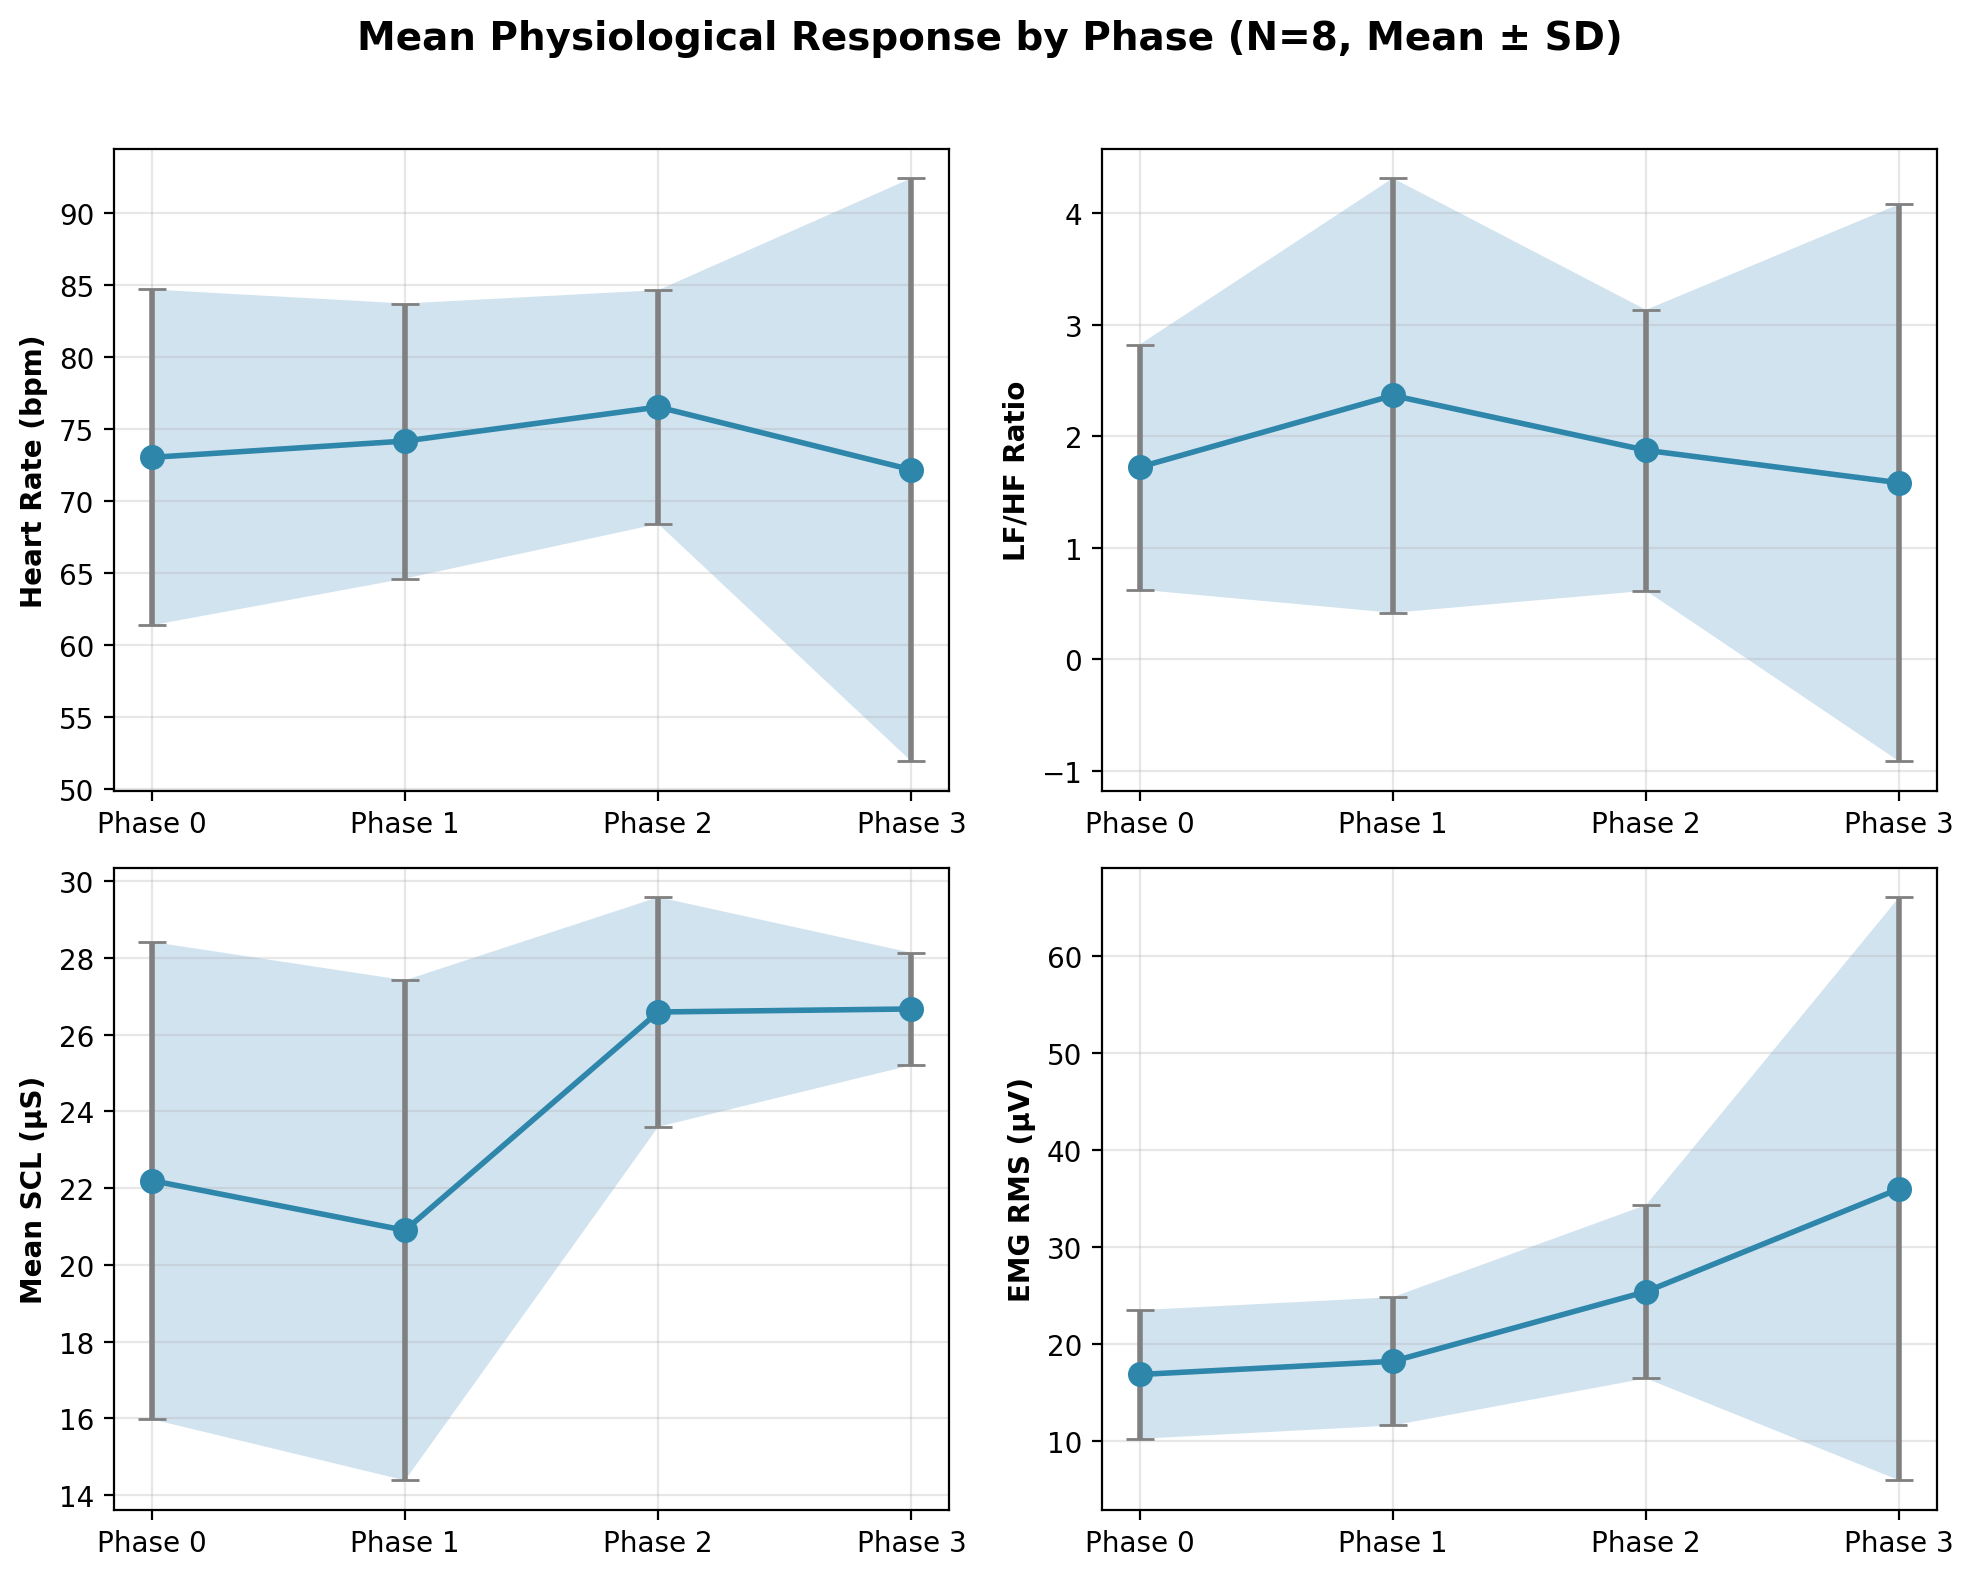
\includegraphics[width=\columnwidth]{fig6_phase_mean.png}
 \caption{Phase別平均生体反応(6名，8セッション，Mean$\pm$SD)}
 \label{fig:phase_mean}
\end{figure}

生体信号からの感情状態の推定においては，20特徴量を用いたLeave-One-Session-Out交差検証の結果，Random Forestが最高精度(Accuracy: 67.7\%，F1: 66.6\%)を示した．Phase~0(安定)のRecall 88\%，Phase~3(追跡)のRecall 71\%と，安定状態と恐怖状態の識別に優れた性能を示した．特徴量の重要度では積分EMG・EMG標準偏差・平均SCL等が上位を占めた．ただし参加者間の精度差(33\%--100\%)が大きく，個人適応機構の必要性が示唆された．

\section{おわりに}
本研究では，VR体験中の感情を生体信号とイベント同期により推定するフレームワークを構築し，参加者実験で有効性を検証した．提案手法はSCLおよびEMGの変化を捉え，フェーズ分類で67.7\%の精度を達成した．また，すくみ反応の検出により，主観評価のみでは把握しにくい没入度の評価可能性を確認した．今後の展望として，加速度データによる動作ノイズ除去，参加者数拡大，スライディングウィンドウ方式による秒単位リアルタイム推定，個人キャリブレーション機構の導入が挙げられる．
本フレームワークの高度化により，VR暴露療法における患者のストレスモニタリングや，ユーザの感情に応じてコンテンツが動的に変化する適応型VR体験の実現が期待される．

\begin{thebibliography}{9}
\bibitem{MarinMorales2018}
J. Marín-Morales et al.: Affective Computing in Virtual Reality: Emotion Recognition from Brain and Heartbeat Dynamics using Wearable Sensors, Scientific Reports, Vol.\,8, No.\,1, pp.\,13657, 2018.

\bibitem{OrozcoMora2024}
C. E. Orozco-Mora et al.: Dynamic Difficulty Adaptation Based on Stress Detection for a Virtual Reality Video Game: A Pilot Study, Electronics, Vol.\,13, No.\,12, pp.\,2324, 2024.

\bibitem{MarinMorales2020}
J. Marín-Morales, C. Llinares, J. Guixeres, and M. Alcañiz: Emotion Recognition in Immersive Virtual Reality: From Statistics to Affective Computing, Sensors, Vol.\,20, No.\,18, pp.\,5163, 2020.
\end{thebibliography}

\end{document}
